% Topic 3.1: Cryptographic Building Blocks
% Self-contained 40-slide presentation for BSC level
\documentclass[11pt,aspectratio=169]{beamer}
\usetheme{Madrid}

% ======================= PACKAGES =======================
\usepackage{graphicx}
\usepackage{booktabs}
\usepackage{adjustbox}
\usepackage{multicol}
\usepackage{amsmath}
\usepackage{amssymb}
\usepackage{tikz}
\usetikzlibrary{arrows,shapes,positioning,shadows,trees}
\usepackage{listings}
\usepackage{xcolor}

% ======================= COLOR DEFINITIONS =======================
% Primary color scheme: Blue/Teal for Digital Finance
\definecolor{dfblue}{RGB}{0,102,204}
\definecolor{dfteal}{RGB}{0,153,153}
\definecolor{dfcyan}{RGB}{51,187,204}
\definecolor{dflightblue}{RGB}{153,204,255}
\definecolor{dflightblue2}{RGB}{173,214,255}
\definecolor{dflightblue3}{RGB}{193,224,255}
\definecolor{dflightblue4}{RGB}{213,234,255}

% Accent colors for finance applications
\definecolor{dfgreen}{RGB}{44, 160, 44}
\definecolor{dfred}{RGB}{214, 39, 40}
\definecolor{dforange}{RGB}{255, 127, 14}
\definecolor{dfgray}{RGB}{127, 127, 127}

% Utility colors
\definecolor{lightgray}{RGB}{240, 240, 240}
\definecolor{midgray}{RGB}{180, 180, 180}
\definecolor{codebg}{RGB}{245, 245, 245}

% ======================= THEME CUSTOMIZATION =======================
% Apply Digital Finance color scheme to Madrid theme
\setbeamercolor{palette primary}{bg=dflightblue3,fg=dfblue}
\setbeamercolor{palette secondary}{bg=dflightblue2,fg=dfblue}
\setbeamercolor{palette tertiary}{bg=dfteal,fg=white}
\setbeamercolor{palette quaternary}{bg=dfblue,fg=white}

\setbeamercolor{structure}{fg=dfblue}
\setbeamercolor{section in toc}{fg=dfblue}
\setbeamercolor{subsection in toc}{fg=dfteal}
\setbeamercolor{title}{fg=dfblue}
\setbeamercolor{frametitle}{fg=dfblue,bg=dflightblue3}
\setbeamercolor{block title}{bg=dflightblue2,fg=dfblue}
\setbeamercolor{block body}{bg=dflightblue4,fg=black}

% Remove navigation symbols for cleaner look
\setbeamertemplate{navigation symbols}{}

% Clean itemize/enumerate
\setbeamertemplate{itemize items}[circle]
\setbeamertemplate{enumerate items}[default]

% Margins for readability
\setbeamersize{text margin left=8mm,text margin right=8mm}

% ======================= LISTINGS CONFIGURATION =======================
% Python code style
\lstdefinestyle{pythonstyle}{
    language=Python,
    basicstyle=\ttfamily\footnotesize,
    keywordstyle=\color{dfblue}\bfseries,
    stringstyle=\color{dforange},
    commentstyle=\color{dfgray}\itshape,
    numberstyle=\tiny\color{dfgray},
    numbers=left,
    numbersep=5pt,
    backgroundcolor=\color{codebg},
    showspaces=false,
    showstringspaces=false,
    showtabs=false,
    frame=single,
    rulecolor=\color{midgray},
    tabsize=4,
    captionpos=b,
    breaklines=true,
    breakatwhitespace=false,
    escapeinside={(*@}{@*)},
    xleftmargin=10pt,
    xrightmargin=10pt
}

% Solidity code style
\lstdefinestyle{soliditystyle}{
    language=Java, % closest approximation
    basicstyle=\ttfamily\footnotesize,
    keywordstyle=\color{dfteal}\bfseries,
    stringstyle=\color{dforange},
    commentstyle=\color{dfgray}\itshape,
    numberstyle=\tiny\color{dfgray},
    numbers=left,
    numbersep=5pt,
    backgroundcolor=\color{codebg},
    showspaces=false,
    showstringspaces=false,
    showtabs=false,
    frame=single,
    rulecolor=\color{midgray},
    tabsize=2,
    captionpos=b,
    breaklines=true,
    breakatwhitespace=false,
    escapeinside={(*@}{@*)},
    xleftmargin=10pt,
    xrightmargin=10pt,
    morekeywords={pragma, contract, function, returns, public, private, view, pure, payable, address, uint256, mapping, event, modifier}
}

% Inline code command
\newcommand{\code}[1]{\texttt{\color{dfblue}#1}}

% ======================= CUSTOM COMMANDS =======================
% Bottom annotation (Madrid-style)
\newcommand{\bottomnote}[1]{%
\vfill
\vspace{-2mm}
\textcolor{dflightblue2}{\rule{\textwidth}{0.4pt}}
\vspace{1mm}
\footnotesize
\textbf{#1}
}

% Compact list spacing
\newcommand{\compactlist}{%
\setlength{\itemsep}{0pt}%
\setlength{\parskip}{0pt}%
\setlength{\parsep}{0pt}%
}

% Chart placeholder
\newcommand{\chartplaceholder}[2][5cm]{%
\begin{center}
\begin{adjustbox}{max width=0.95\textwidth, max height=#1}
\framebox[\textwidth][c]{%
\rule{0pt}{#1}%
\textcolor{midgray}{[#2]}%
}
\end{adjustbox}
\end{center}
}

% ======================= FINANCE NOTATION MACROS =======================
% Probability and statistics
\newcommand{\E}{\mathbb{E}} % Expected value
\newcommand{\Var}{\mathrm{Var}} % Variance
\newcommand{\Cov}{\mathrm{Cov}} % Covariance
\newcommand{\Prob}{\mathbb{P}} % Probability

% Distributions
\newcommand{\Normal}{\mathcal{N}} % Normal distribution
\newcommand{\Uniform}{\mathcal{U}} % Uniform distribution

% Returns and prices
\newcommand{\Ret}{R} % Return
\newcommand{\LogRet}{r} % Log return
\newcommand{\Price}{S} % Price/Stock price
\newcommand{\Strike}{K} % Strike price

% Options and derivatives
\newcommand{\CallPrice}{C} % Call option price
\newcommand{\PutPrice}{P} % Put option price
\newcommand{\Greeks}[1]{\mathit{#1}} % Greek letters

% Risk measures
\newcommand{\VaR}{\mathrm{VaR}} % Value at Risk
\newcommand{\CVaR}{\mathrm{CVaR}} % Conditional VaR
\newcommand{\Sharpe}{\mathrm{SR}} % Sharpe Ratio

% Time series
\newcommand{\AR}{\mathrm{AR}} % Autoregressive
\newcommand{\MA}{\mathrm{MA}} % Moving average
\newcommand{\GARCH}{\mathrm{GARCH}} % GARCH

% Blockchain/Crypto
\newcommand{\Hash}{\mathrm{Hash}} % Hash function
\newcommand{\Block}{\mathcal{B}} % Block
\newcommand{\Chain}{\mathcal{C}} % Chain

% Real numbers, integers
\newcommand{\R}{\mathbb{R}}
\newcommand{\Z}{\mathbb{Z}}
\newcommand{\N}{\mathbb{N}}

% ======================= TIKZ STYLES =======================
% Styles for finance-related diagrams
\tikzstyle{process} = [rectangle, minimum width=3cm, minimum height=1cm, text centered, draw=dfblue, fill=dflightblue4, thick]
\tikzstyle{decision} = [diamond, minimum width=3cm, minimum height=1cm, text centered, draw=dfteal, fill=dflightblue4, thick]
\tikzstyle{arrow} = [thick,->,>=stealth,color=dfblue]
\tikzstyle{blockchain} = [rectangle, rounded corners, minimum width=2.5cm, minimum height=1cm, text centered, draw=dfteal, fill=dflightblue3, thick]
\tikzstyle{transaction} = [circle, minimum size=0.8cm, text centered, draw=dforange, fill=dflightblue4, thick]

% ======================= FOOTER TEMPLATE =======================
\setbeamertemplate{footline}{
    \hbox{\begin{beamercolorbox}[wd=\paperwidth,ht=2.5ex,dp=1ex,leftskip=.5em,rightskip=.5em]{author in head/foot}
    \tiny
    \textbf{Digital Finance} \hfill
    Joerg Osterrieder \hfill
    \insertdate \hfill
    Page \insertframenumber{} / \inserttotalframenumber
    \end{beamercolorbox}}
}

% ======================= SECTION DIVIDER TEMPLATE =======================
\AtBeginSection[]{
\begin{frame}[plain]
\vfill
\centering
\begin{beamercolorbox}[sep=12pt,center]{title}
\usebeamerfont{title}\LARGE\insertsection\par
\end{beamercolorbox}
\vfill
\end{frame}
}


% Additional TikZ libraries
\usetikzlibrary{chains,calc,decorations.pathreplacing,fit,backgrounds}

% Custom styles for cryptography diagrams
\tikzstyle{hashbox} = [rectangle, rounded corners, minimum width=2cm, minimum height=0.8cm, text centered, draw=dfteal, fill=dflightblue3, thick, font=\footnotesize]
\tikzstyle{databox} = [rectangle, minimum width=2.5cm, minimum height=0.6cm, text centered, draw=dfblue, fill=dflightblue4, thick, font=\footnotesize]
\tikzstyle{keybox} = [rectangle, rounded corners, minimum width=2cm, minimum height=0.6cm, text centered, draw=dforange, fill=dflightblue4, thick, font=\footnotesize]

% ======================= DOCUMENT INFO =======================
\title[Topic 3.1: Cryptographic Building Blocks]{Topic 3.1: Cryptographic Building Blocks}
\subtitle{Hashing, Keys, and Digital Signatures}
\author{Joerg Osterrieder}
\institute{Digital Finance}
\date{2025}

\begin{document}

% =======================================================================
% SLIDE 1: Title Slide
% =======================================================================
\begin{frame}[plain]
\titlepage
\end{frame}

% =======================================================================
% SLIDE 2: Learning Objectives
% =======================================================================
\begin{frame}{Learning Objectives}
By the end of this topic, you will be able to:

\vspace{3mm}
\begin{enumerate}
\item \textbf{Explain} what cryptographic hash functions are and their essential properties
\vspace{2mm}
\item \textbf{Describe} how public-key cryptography enables secure identity without a central authority
\vspace{2mm}
\item \textbf{Understand} how digital signatures provide authentication, integrity, and non-repudiation
\vspace{2mm}
\item \textbf{Connect} these three primitives to how blockchain systems establish trust
\vspace{2mm}
\item \textbf{Apply} these concepts in hands-on exercises using Python
\end{enumerate}

\vspace{5mm}
\begin{block}{Why This Matters}
Cryptography is the foundation that allows blockchain to replace institutional trust with mathematical proof.
\end{block}
\end{frame}

% =======================================================================
% SLIDE 3: Prerequisites/Background (Part 1)
% =======================================================================
\begin{frame}{What is Cryptography?}
\begin{columns}[T]
\begin{column}{0.55\textwidth}
\textbf{Definition:} The science of secure communication in the presence of adversaries.

\vspace{3mm}
\textbf{Everyday Examples:}
\begin{itemize}
\item \textbf{HTTPS} -- Secure websites (the padlock icon)
\item \textbf{WhatsApp} -- End-to-end encrypted messages
\item \textbf{ATM PINs} -- Encrypted card data
\item \textbf{Passwords} -- Stored as hashes, not plaintext
\end{itemize}

\vspace{3mm}
\textcolor{dfblue}{\textbf{Key Insight:}} You already use cryptography daily!
\end{column}
\begin{column}{0.42\textwidth}
\begin{center}
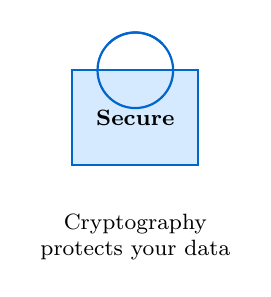
\begin{tikzpicture}[scale=0.8]
% Lock icon
\draw[thick, dfblue, fill=dflightblue4] (0,0) rectangle (2,1.5);
\draw[thick, dfblue] (1,1.5) circle (0.6);
\draw[thick, dfblue] (1,1.5) ++(135:0.6) arc (135:45:0.6);
\node at (1,0.75) {\footnotesize \textbf{Secure}};

% Labels
\node[below=0.5cm of {(1,0)}, text width=2.5cm, align=center, font=\footnotesize] {
Cryptography protects your data
};
\end{tikzpicture}
\end{center}

\vspace{3mm}
\textbf{In This Topic:}\\
We focus on \textit{what} cryptographic tools guarantee, not the complex math behind them.
\end{column}
\end{columns}
\end{frame}

% =======================================================================
% SLIDE 4: Prerequisites/Background (Part 2)
% =======================================================================
\begin{frame}{The Trust Problem: Why Cryptography Matters for Finance}
\begin{columns}[T]
\begin{column}{0.5\textwidth}
\textbf{Traditional Trust Model}
\begin{itemize}
\item Banks verify your identity
\item Courts enforce contracts
\item Governments back currency
\item Intermediaries everywhere
\end{itemize}
\vspace{3mm}
\textcolor{dfred}{Problem: Single points of failure}
\end{column}
\begin{column}{0.5\textwidth}
\textbf{Cryptographic Trust Model}
\begin{itemize}
\item Mathematics verifies identity
\item Code enforces agreements
\item Network backs value
\item Trust is distributed
\end{itemize}
\vspace{3mm}
\textcolor{dfgreen}{Solution: Trust through verification}
\end{column}
\end{columns}

\vspace{5mm}
\begin{center}
\fbox{\parbox{0.8\textwidth}{\centering
\textbf{Key Insight:} Cryptography lets us replace ``trust me'' with ``verify this''
}}
\end{center}
\end{frame}

% =======================================================================
% SLIDE 5: Three Cryptographic Primitives Overview
% =======================================================================
\begin{frame}{Three Cryptographic Primitives}
\begin{center}
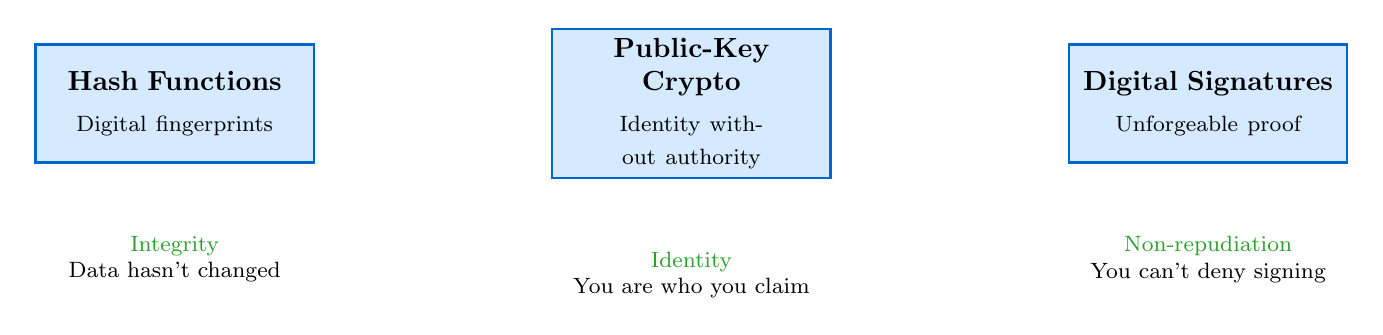
\begin{tikzpicture}[node distance=3cm]
% Three main boxes
\node[process, minimum width=3.5cm, minimum height=1.5cm, text width=3.3cm, align=center] (hash) {
\textbf{Hash Functions}\\[1mm]
\footnotesize Digital fingerprints
};
\node[process, minimum width=3.5cm, minimum height=1.5cm, text width=3.3cm, align=center, right=of hash] (keys) {
\textbf{Public-Key Crypto}\\[1mm]
\footnotesize Identity without authority
};
\node[process, minimum width=3.5cm, minimum height=1.5cm, text width=3.3cm, align=center, right=of keys] (sigs) {
\textbf{Digital Signatures}\\[1mm]
\footnotesize Unforgeable proof
};

% What they guarantee
\node[below=0.8cm of hash, text width=3.5cm, align=center, font=\footnotesize] {
\textcolor{dfgreen}{Integrity}\\
Data hasn't changed
};
\node[below=0.8cm of keys, text width=3.5cm, align=center, font=\footnotesize] {
\textcolor{dfgreen}{Identity}\\
You are who you claim
};
\node[below=0.8cm of sigs, text width=3.5cm, align=center, font=\footnotesize] {
\textcolor{dfgreen}{Non-repudiation}\\
You can't deny signing
};
\end{tikzpicture}
\end{center}

\vspace{3mm}
\textbf{Focus:} What these tools \textit{guarantee}, not how the math works

\bottomnote{These three primitives are the atoms of decentralized trust}
\end{frame}

% =======================================================================
% SLIDE 6: What is a Hash Function?
% =======================================================================
\begin{frame}{What is a Hash Function?}
\textbf{Definition:} A hash function takes \textit{any} input and produces a fixed-size output called a \textbf{hash} (or digest).

\vspace{3mm}
\begin{center}
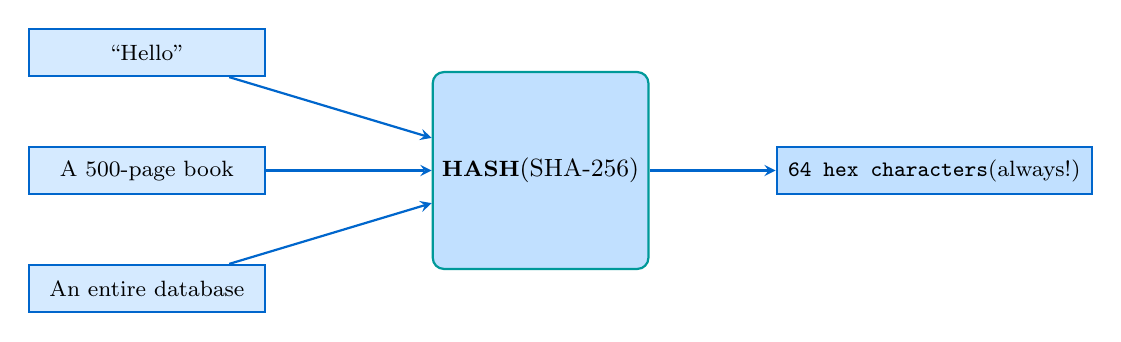
\begin{tikzpicture}
% Input examples
\node[databox, minimum width=3cm] (in1) at (0,1.5) {``Hello''};
\node[databox, minimum width=3cm] (in2) at (0,0) {A 500-page book};
\node[databox, minimum width=3cm] (in3) at (0,-1.5) {An entire database};

% Hash function
\node[hashbox, minimum width=2.5cm, minimum height=2.5cm] (hash) at (5,0) {\textbf{HASH}\\\small (SHA-256)};

% Output
\node[databox, minimum width=4cm, fill=dflightblue3] (out) at (10,0) {\texttt{64 hex characters}\\(always!)};

% Arrows
\draw[arrow] (in1) -- (hash);
\draw[arrow] (in2) -- (hash);
\draw[arrow] (in3) -- (hash);
\draw[arrow] (hash) -- (out);
\end{tikzpicture}
\end{center}

\vspace{3mm}
\textbf{Think of it like:} A fingerprint machine for data
\begin{itemize}
\item Any person $\rightarrow$ unique fingerprint (fixed size)
\item Any data $\rightarrow$ unique hash (fixed size: 256 bits)
\end{itemize}
\end{frame}

% =======================================================================
% SLIDE 7: Hash Functions - Digital Fingerprints
% =======================================================================
\begin{frame}{Hash Functions: Digital Fingerprints}
\begin{center}
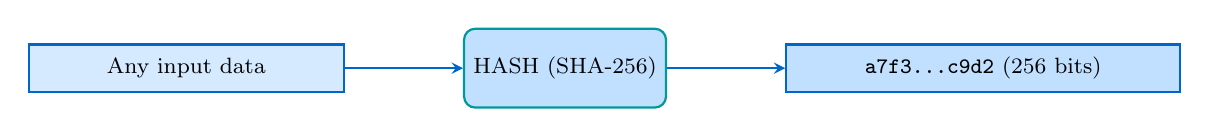
\begin{tikzpicture}
% Input
\node[databox, minimum width=4cm] (input) {Any input data};
% Hash function
\node[hashbox, right=1.5cm of input, minimum width=2.5cm, minimum height=1cm] (hash) {HASH (SHA-256)};
% Output
\node[databox, right=1.5cm of hash, minimum width=5cm, fill=dflightblue3] (output) {\texttt{a7f3...c9d2} (256 bits)};

\draw[arrow] (input) -- (hash);
\draw[arrow] (hash) -- (output);
\end{tikzpicture}
\end{center}

\vspace{5mm}
\begin{tabular}{ll}
\textcolor{dfblue}{\textbf{Deterministic:}} & Same input $\rightarrow$ same output, always\\[2mm]
\textcolor{dfblue}{\textbf{One-way:}} & Cannot reverse to find input\\[2mm]
\textcolor{dfblue}{\textbf{Collision-resistant:}} & Practically impossible to find two inputs with same hash\\[2mm]
\textcolor{dfblue}{\textbf{Avalanche effect:}} & Tiny change $\rightarrow$ completely different output\\
\end{tabular}
\end{frame}

% =======================================================================
% SLIDE 8: The Five Properties Explained
% =======================================================================
\begin{frame}{Five Essential Properties of Hash Functions}
\begin{enumerate}
\item \textbf{Deterministic}\\
\textcolor{dfgray}{\small Hash(``Bitcoin'') today = Hash(``Bitcoin'') tomorrow = Hash(``Bitcoin'') forever}

\vspace{2mm}
\item \textbf{Fixed Output Size}\\
\textcolor{dfgray}{\small SHA-256 always produces 256 bits (64 hex characters), regardless of input size}

\vspace{2mm}
\item \textbf{One-Way (Preimage Resistant)}\\
\textcolor{dfgray}{\small Given a hash, you cannot compute the original input}

\vspace{2mm}
\item \textbf{Collision Resistant}\\
\textcolor{dfgray}{\small Practically impossible to find two different inputs with the same hash}

\vspace{2mm}
\item \textbf{Avalanche Effect}\\
\textcolor{dfgray}{\small Change 1 bit of input $\rightarrow$ approximately 50\% of output bits change}
\end{enumerate}

\vspace{3mm}
\begin{block}{Why These Matter}
Together, these properties make hashes reliable ``digital fingerprints'' for data integrity.
\end{block}
\end{frame}

% =======================================================================
% SLIDE 9: The Avalanche Effect Visualized
% =======================================================================
\begin{frame}{The Avalanche Effect Visualized}
\begin{center}
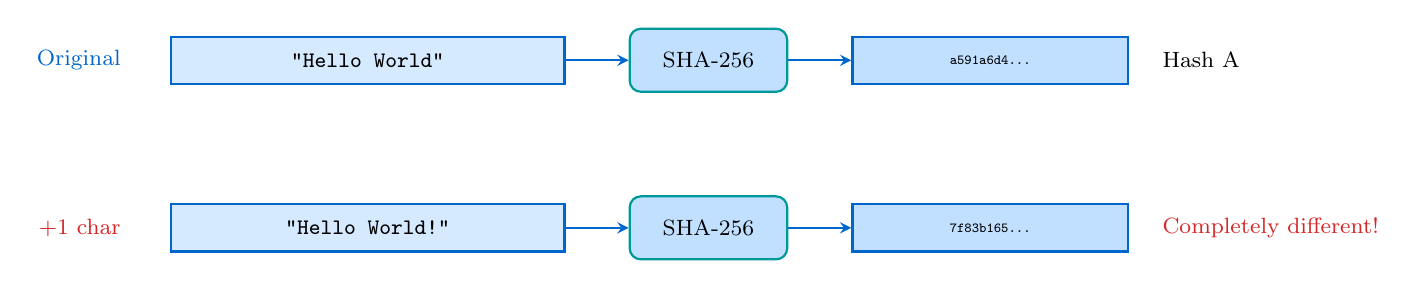
\begin{tikzpicture}[node distance=0.8cm]
% Example 1
\node[databox, minimum width=5cm] (in1) {\texttt{"Hello World"}};
\node[hashbox, right=0.8cm of in1, minimum width=2cm] (h1) {SHA-256};
\node[databox, right=0.8cm of h1, minimum width=3.5cm, fill=dflightblue3, font=\tiny\ttfamily] (out1) {a591a6d4...};
\draw[arrow] (in1) -- (h1);
\draw[arrow] (h1) -- (out1);

% Example 2 - tiny change
\node[databox, minimum width=5cm, below=1.5cm of in1] (in2) {\texttt{"Hello World!"}};
\node[hashbox, right=0.8cm of in2, minimum width=2cm] (h2) {SHA-256};
\node[databox, right=0.8cm of h2, minimum width=3.5cm, fill=dflightblue3, font=\tiny\ttfamily] (out2) {7f83b165...};
\draw[arrow] (in2) -- (h2);
\draw[arrow] (h2) -- (out2);

% Annotations
\node[left=0.5cm of in1, font=\footnotesize, text=dfblue] {Original};
\node[left=0.5cm of in2, font=\footnotesize, text=dfred] {+1 char};
\node[right=0.3cm of out1, font=\footnotesize] {Hash A};
\node[right=0.3cm of out2, font=\footnotesize, text=dfred] {Completely different!};
\end{tikzpicture}
\end{center}

\vspace{5mm}
\textbf{Why this matters for blockchain:}
\begin{itemize}
\item Change one transaction $\rightarrow$ entire block hash changes
\item This change cascades through all subsequent blocks
\item Tampering becomes immediately detectable
\end{itemize}
\end{frame}

% =======================================================================
% SLIDE 10: SHA-256 Security Numbers
% =======================================================================
\begin{frame}{How Secure is SHA-256?}
\textbf{SHA-256 produces $2^{256}$ possible outputs.}

\vspace{3mm}
How big is that number?

\begin{center}
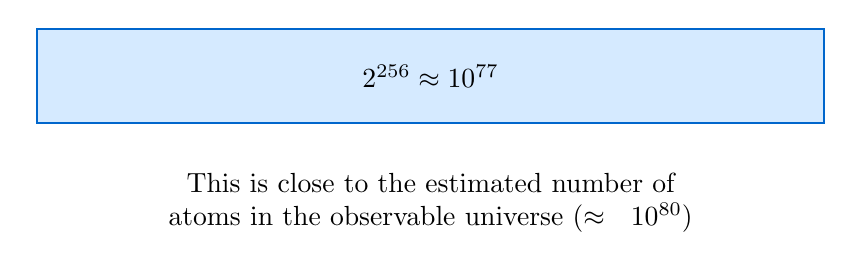
\begin{tikzpicture}
\node[process, minimum width=10cm, minimum height=1.2cm] (box) {
$2^{256} \approx 10^{77}$
};
\node[below=0.5cm of box, text width=10cm, align=center] {
This is close to the estimated number of atoms in the observable universe ($\approx 10^{80}$)
};
\end{tikzpicture}
\end{center}

\vspace{3mm}
\textbf{To find a collision by brute force:}
\begin{itemize}
\item Even trying 1 billion hashes per second
\item Using every computer on Earth
\item Would take longer than the age of the universe
\end{itemize}

\vspace{3mm}
\begin{block}{Practical Security}
SHA-256 is considered cryptographically secure for all practical purposes.
\end{block}
\end{frame}

% =======================================================================
% SLIDE 11: Hash Functions in Blockchain
% =======================================================================
\begin{frame}{What Hash Functions Guarantee}
\begin{columns}[T]
\begin{column}{0.55\textwidth}
\textbf{Use Cases in Blockchain}
\begin{itemize}\compactlist
\item \textbf{Data integrity:} Verify nothing changed
\item \textbf{Block linking:} Each block contains hash of previous
\item \textbf{Transaction IDs:} Unique identifier for every transaction
\item \textbf{Mining puzzles:} Finding hashes with specific properties
\item \textbf{Merkle trees:} Efficiently verify large data sets
\end{itemize}
\end{column}
\begin{column}{0.42\textwidth}
\begin{center}
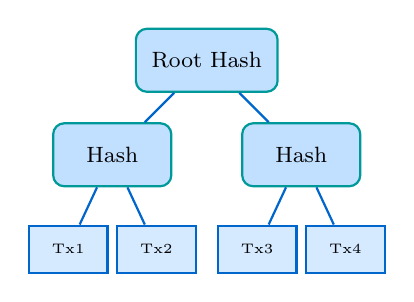
\begin{tikzpicture}[scale=0.8]
% Merkle tree
\node[hashbox, minimum width=1.8cm] (root) at (0,3) {Root Hash};
\node[hashbox, minimum width=1.5cm] (h1) at (-1.5,1.5) {Hash};
\node[hashbox, minimum width=1.5cm] (h2) at (1.5,1.5) {Hash};
\node[databox, minimum width=1cm, font=\tiny] (t1) at (-2.2,0) {Tx1};
\node[databox, minimum width=1cm, font=\tiny] (t2) at (-0.8,0) {Tx2};
\node[databox, minimum width=1cm, font=\tiny] (t3) at (0.8,0) {Tx3};
\node[databox, minimum width=1cm, font=\tiny] (t4) at (2.2,0) {Tx4};

\draw[thick, dfblue] (t1) -- (h1);
\draw[thick, dfblue] (t2) -- (h1);
\draw[thick, dfblue] (t3) -- (h2);
\draw[thick, dfblue] (t4) -- (h2);
\draw[thick, dfblue] (h1) -- (root);
\draw[thick, dfblue] (h2) -- (root);
\end{tikzpicture}

\footnotesize\textbf{Merkle Tree}\\
\textit{Like a family tree where you can verify any member by checking their parents}\\[1mm]
Verify any transaction with $O(\log n)$ hashes
\end{center}
\end{column}
\end{columns}

\vspace{3mm}
\begin{block}{The Guarantee}
If two hashes match, the data is identical (with overwhelming probability).
\end{block}
\end{frame}

% =======================================================================
% SLIDE 12: Merkle Trees Explained
% =======================================================================
\begin{frame}{Merkle Trees: Efficient Data Verification}
\textbf{Problem:} How do you verify one transaction out of thousands without downloading everything?

\vspace{1mm}
\textit{Like verifying one page of a book by checking chapter summaries -- you don't need to read every page}

\vspace{2mm}
\begin{center}
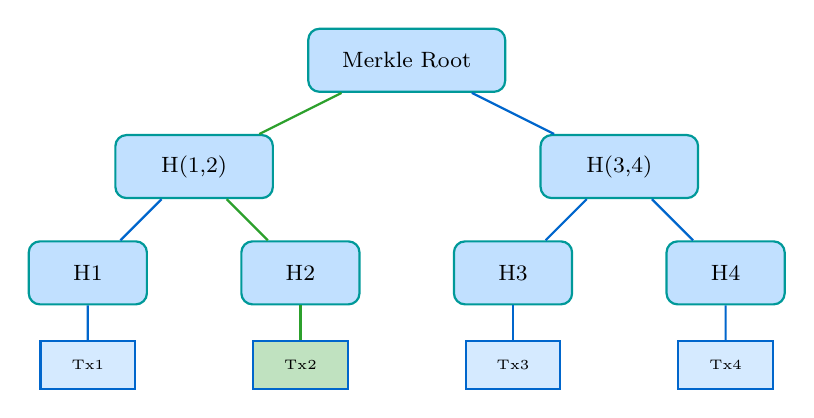
\begin{tikzpicture}[scale=0.9]
% Root
\node[hashbox, minimum width=2.5cm] (root) at (0,4) {Merkle Root};

% Level 1
\node[hashbox, minimum width=2cm] (h12) at (-3,2.5) {H(1,2)};
\node[hashbox, minimum width=2cm] (h34) at (3,2.5) {H(3,4)};

% Level 2
\node[hashbox, minimum width=1.5cm] (h1) at (-4.5,1) {H1};
\node[hashbox, minimum width=1.5cm] (h2) at (-1.5,1) {H2};
\node[hashbox, minimum width=1.5cm] (h3) at (1.5,1) {H3};
\node[hashbox, minimum width=1.5cm] (h4) at (4.5,1) {H4};

% Transactions
\node[databox, minimum width=1.2cm, font=\tiny] (t1) at (-4.5,-0.3) {Tx1};
\node[databox, minimum width=1.2cm, font=\tiny, fill=dfgreen!30] (t2) at (-1.5,-0.3) {Tx2};
\node[databox, minimum width=1.2cm, font=\tiny] (t3) at (1.5,-0.3) {Tx3};
\node[databox, minimum width=1.2cm, font=\tiny] (t4) at (4.5,-0.3) {Tx4};

% Connections
\draw[thick, dfblue] (t1) -- (h1);
\draw[thick, dfgreen] (t2) -- (h2);
\draw[thick, dfblue] (t3) -- (h3);
\draw[thick, dfblue] (t4) -- (h4);
\draw[thick, dfblue] (h1) -- (h12);
\draw[thick, dfgreen] (h2) -- (h12);
\draw[thick, dfblue] (h3) -- (h34);
\draw[thick, dfblue] (h4) -- (h34);
\draw[thick, dfgreen] (h12) -- (root);
\draw[thick, dfblue] (h34) -- (root);
\end{tikzpicture}
\end{center}

\vspace{2mm}
\textbf{To verify Tx2:} Only need H1, H(3,4), and Merkle Root (3 items, not 4 transactions)

\bottomnote{With 1 million transactions, you only need about 20 hashes to verify any single one}
\end{frame}

% =======================================================================
% SLIDE 13: Introduction to Public-Key Cryptography
% =======================================================================
\begin{frame}{Introduction to Public-Key Cryptography}
\textbf{The Problem:} How can two strangers communicate securely without meeting first to exchange a secret password?

\vspace{5mm}
\textbf{Traditional (Symmetric) Encryption:}
\begin{itemize}
\item Same key encrypts and decrypts
\item Problem: How do you safely share the key?
\end{itemize}

\vspace{3mm}
\textbf{Public-Key (Asymmetric) Solution:}
\begin{itemize}
\item Two mathematically related keys
\item One key encrypts $\rightarrow$ only the other decrypts
\item Share one key publicly, keep the other secret
\end{itemize}

\vspace{5mm}
\begin{center}
\fbox{\parbox{0.7\textwidth}{\centering
\textbf{Breakthrough (1976):} Diffie, Hellman, and later RSA showed this was mathematically possible
}}
\end{center}
\end{frame}

% =======================================================================
% SLIDE 14: Public-Key Cryptography Key Generation
% =======================================================================
\begin{frame}{Public-Key Cryptography: Identity Without Authority}
\begin{center}
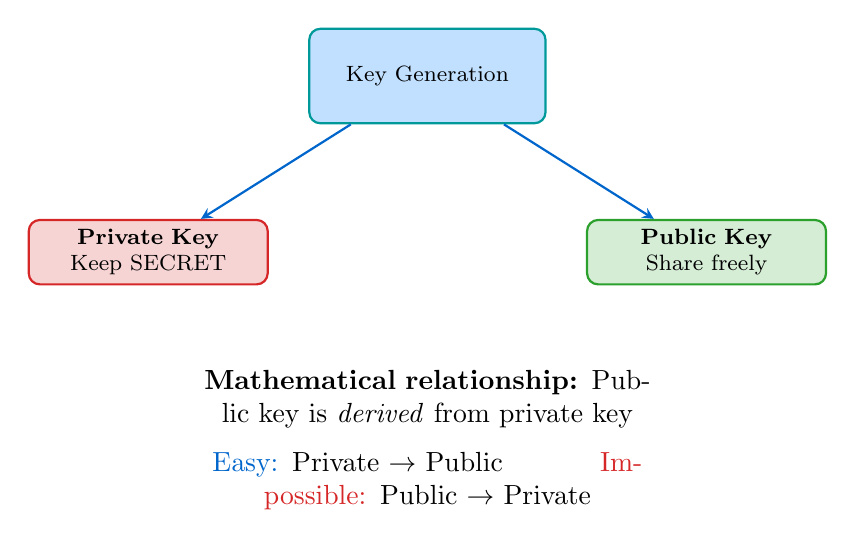
\begin{tikzpicture}[node distance=1cm]
% Key generation
\node[hashbox, minimum width=3cm, minimum height=1.2cm] (gen) {Key Generation};

% Private key
\node[keybox, below left=1.2cm and 0.5cm of gen, fill=dfred!20, draw=dfred, minimum width=3cm, text width=2.8cm, align=center] (priv) {
\textbf{Private Key}\\
\footnotesize Keep SECRET
};

% Public key
\node[keybox, below right=1.2cm and 0.5cm of gen, fill=dfgreen!20, draw=dfgreen, minimum width=3cm, text width=2.8cm, align=center] (pub) {
\textbf{Public Key}\\
\footnotesize Share freely
};

\draw[arrow] (gen) -- (priv);
\draw[arrow] (gen) -- (pub);

% Relationship
\node[below=3cm of gen, text width=9cm, align=center] {
\textbf{Mathematical relationship:} Public key is \textit{derived} from private key\\[2mm]
\textcolor{dfblue}{Easy:} Private $\rightarrow$ Public \hspace{1cm}
\textcolor{dfred}{Impossible:} Public $\rightarrow$ Private
};
\end{tikzpicture}
\end{center}
\end{frame}

% =======================================================================
% SLIDE 15: How Public-Key Crypto Works
% =======================================================================
\begin{frame}{Public-Key Cryptography: How It Works}
\begin{center}
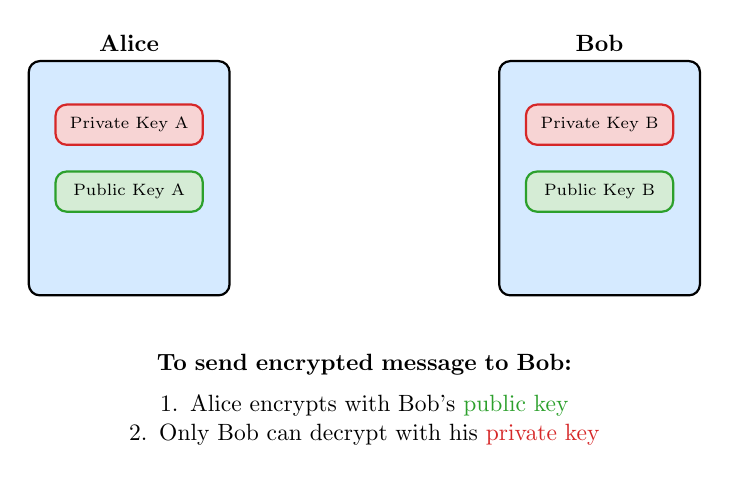
\begin{tikzpicture}[node distance=0.5cm, scale=0.85, transform shape]
% Alice
\node[draw, thick, rounded corners, minimum width=3cm, minimum height=3.5cm, fill=dflightblue4] (alice) {};
\node[above=0mm of alice.north, font=\bfseries] {Alice};
\node[keybox, fill=dfred!20, draw=dfred, minimum width=2.2cm, font=\scriptsize] at ($(alice.center) + (0,0.8)$) {Private Key A};
\node[keybox, fill=dfgreen!20, draw=dfgreen, minimum width=2.2cm, font=\scriptsize] at ($(alice.center) + (0,-0.2)$) {Public Key A};

% Bob
\node[draw, thick, rounded corners, minimum width=3cm, minimum height=3.5cm, fill=dflightblue4, right=4cm of alice] (bob) {};
\node[above=0mm of bob.north, font=\bfseries] {Bob};
\node[keybox, fill=dfred!20, draw=dfred, minimum width=2.2cm, font=\scriptsize] at ($(bob.center) + (0,0.8)$) {Private Key B};
\node[keybox, fill=dfgreen!20, draw=dfgreen, minimum width=2.2cm, font=\scriptsize] at ($(bob.center) + (0,-0.2)$) (bpub) {Public Key B};

% Message flow
\node[below=2.5cm of $(alice)!0.5!(bob)$, text width=8cm, align=center] {
\textbf{To send encrypted message to Bob:}\\[2mm]
1. Alice encrypts with Bob's \textcolor{dfgreen}{public key}\\
2. Only Bob can decrypt with his \textcolor{dfred}{private key}
};
\end{tikzpicture}
\end{center}

\vspace{2mm}
\textbf{Key insight:} Only the person with the private key can decrypt
\end{frame}

% =======================================================================
% SLIDE 16: The Mathematical Foundation (Simplified)
% =======================================================================
\begin{frame}{The Mathematical Intuition (No Math Required!)}
\textbf{Analogy: The Padlock and Key}

\vspace{3mm}
\begin{columns}[T]
\begin{column}{0.5\textwidth}
\textbf{Traditional Lock}
\begin{itemize}
\item Same key locks and unlocks
\item Must physically give key to someone
\item If copied, security is broken
\end{itemize}
\end{column}
\begin{column}{0.5\textwidth}
\textbf{Public-Key ``Lock''}
\begin{itemize}
\item Public key = open padlock (share freely)
\item Private key = the only key that opens it
\item Anyone can lock (encrypt), only you can open (decrypt)
\end{itemize}
\end{column}
\end{columns}

\vspace{5mm}
\begin{center}

\begin{tikzpicture}
\node[databox, minimum width=3cm] (msg) {Message};
\node[right=0.5cm of msg] (plus) {$+$};
\node[keybox, fill=dfgreen!20, draw=dfgreen, right=0.5cm of plus] (pub) {Public Key};
\node[right=0.5cm of pub] (eq) {$\rightarrow$};
\node[databox, fill=dforange!30, right=0.5cm of eq] (enc) {Encrypted};
\node[right=0.5cm of enc] (plus2) {$+$};
\node[keybox, fill=dfred!20, draw=dfred, right=0.5cm of plus2] (priv) {Private Key};
\node[right=0.5cm of priv] (eq2) {$\rightarrow$};
\node[databox, right=0.5cm of eq2] (dec) {Message};
\end{tikzpicture}
\end{center}
\end{frame}

% =======================================================================
% SLIDE 17: From Public Key to Blockchain Address
% =======================================================================
\begin{frame}{From Public Key to Blockchain Address}
\begin{center}
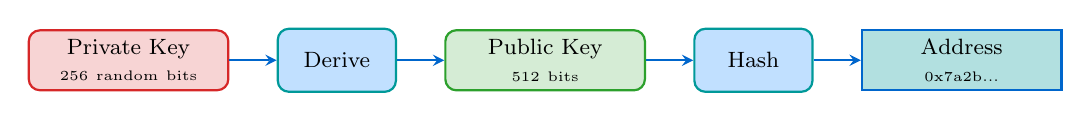
\begin{tikzpicture}[node distance=0.4cm]
% Flow
\node[keybox, fill=dfred!20, draw=dfred, minimum width=2.5cm, text width=2.3cm, align=center] (priv) {Private Key\\{\tiny 256 random bits}};
\node[hashbox, right=0.6cm of priv, minimum width=1.5cm] (derive) {Derive};
\node[keybox, fill=dfgreen!20, draw=dfgreen, minimum width=2.5cm, text width=2.3cm, align=center, right=0.6cm of derive] (pub) {Public Key\\{\tiny 512 bits}};
\node[hashbox, right=0.6cm of pub, minimum width=1.5cm] (hash) {Hash};
\node[databox, fill=dfteal!30, minimum width=2.5cm, text width=2.3cm, align=center, right=0.6cm of hash] (addr) {Address\\{\tiny 0x7a2b...}};

\draw[arrow] (priv) -- (derive);
\draw[arrow] (derive) -- (pub);
\draw[arrow] (pub) -- (hash);
\draw[arrow] (hash) -- (addr);
\end{tikzpicture}
\end{center}

\vspace{5mm}
\begin{columns}[T]
\begin{column}{0.48\textwidth}
\textbf{What You Control}
\begin{itemize}
\item Private key = your identity
\item Whoever has it controls the funds
\item \textcolor{dfred}{Lose it = lose everything}
\item \textcolor{dfred}{Share it = share everything}
\end{itemize}
\end{column}
\begin{column}{0.48\textwidth}
\textbf{What You Share}
\begin{itemize}
\item Address = your ``account number''
\item Safe to share publicly
\item Used to receive payments
\item Cannot derive private key from it
\end{itemize}
\end{column}
\end{columns}

\bottomnote{``Not your keys, not your coins'' -- a fundamental principle of crypto}
\end{frame}

% =======================================================================
% SLIDE 18: ECDSA vs RSA
% =======================================================================
\begin{frame}{Elliptic Curve Cryptography in Blockchain}
\textbf{Why don't blockchains use RSA?}

\vspace{2mm}
\textit{Two different mathematical approaches to creating unforgeable digital signatures:}

\begin{itemize}
\item \textbf{RSA:} Based on factoring large prime numbers
\item \textbf{ECDSA (Elliptic Curve Digital Signature Algorithm):} Based on elliptic curve mathematics
\end{itemize}

\vspace{2mm}
\begin{center}
\begin{tabular}{lcc}
\toprule
\textbf{Property} & \textbf{RSA} & \textbf{ECDSA (secp256k1)} \\
\midrule
Key Size (equiv. security) & 3072 bits & 256 bits \\
Signature Size & Large & Small \\
Speed & Slower & Faster \\
Used by Bitcoin/Ethereum & No & Yes \\
\bottomrule
\end{tabular}
\end{center}

\vspace{3mm}
\textbf{secp256k1:} The specific mathematical curve Bitcoin and Ethereum use for signatures
\begin{itemize}
\item Provides 256-bit security (more combinations than atoms in the observable universe) with smaller keys
\item Smaller signatures = lower transaction fees
\item Well-studied and standardized
\end{itemize}

\bottomnote{In NB05, we use RSA for simplicity, but real blockchains use ECDSA with secp256k1}
\end{frame}

% =======================================================================
% SLIDE 19: Introduction to Digital Signatures
% =======================================================================
\begin{frame}{What is a Digital Signature?}
\textbf{Definition:} A mathematical scheme that proves:
\begin{enumerate}
\item \textbf{Who} created or approved a message (authentication)
\item That the message \textbf{hasn't been changed} (integrity)
\item The signer \textbf{can't deny} signing (non-repudiation)
\end{enumerate}

\vspace{5mm}
\textbf{Physical vs Digital Signatures:}

\begin{center}
\begin{tabular}{lcc}
\toprule
\textbf{Property} & \textbf{Handwritten} & \textbf{Digital} \\
\midrule
Can be forged? & Yes & Practically no \\
Tied to document? & No & Yes (any change invalidates) \\
Remotely verifiable? & No & Yes \\
Provably unique? & No & Yes \\
\bottomrule
\end{tabular}
\end{center}

\vspace{3mm}
\textcolor{dfblue}{\textbf{Key Point:}} Digital signatures are \textit{stronger} than handwritten ones!
\end{frame}

% =======================================================================
% SLIDE 20: Digital Signatures - How They Work
% =======================================================================
\begin{frame}{Digital Signatures: Unforgeable Proof}
\begin{center}
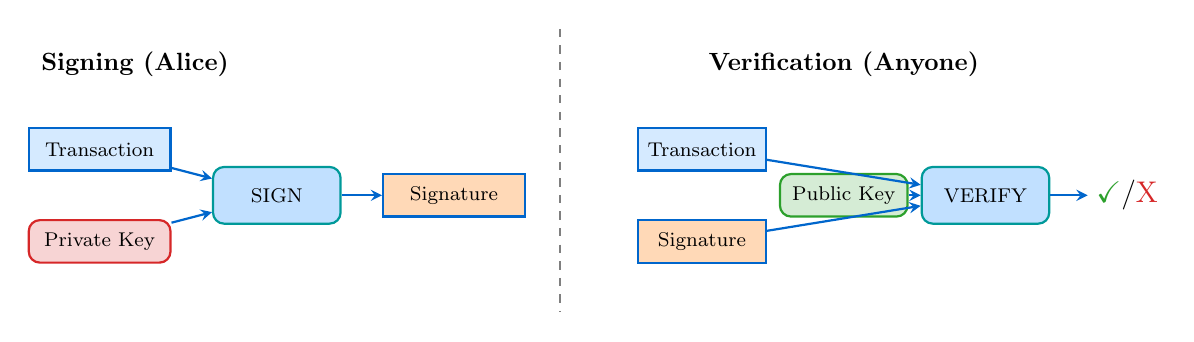
\begin{tikzpicture}[node distance=0.5cm, scale=0.9, transform shape]
% Signing process
\node[font=\bfseries] at (-4.5, 2) {Signing (Alice)};

\node[databox, minimum width=2cm] (msg) at (-5,0.8) {Transaction};
\node[keybox, fill=dfred!20, draw=dfred, minimum width=2cm] (key) at (-5,-0.5) {Private Key};
\node[hashbox, minimum width=1.8cm] (sign) at (-2.5,0.15) {SIGN};
\node[databox, fill=dforange!30, minimum width=2cm] (sig) at (0,0.15) {Signature};

\draw[arrow] (msg) -- (sign);
\draw[arrow] (key) -- (sign);
\draw[arrow] (sign) -- (sig);

% Verification process
\node[font=\bfseries] at (5.5, 2) {Verification (Anyone)};

\node[databox, minimum width=1.8cm] (msg2) at (3.5,0.8) {Transaction};
\node[databox, fill=dforange!30, minimum width=1.8cm] (sig2) at (3.5,-0.5) {Signature};
\node[keybox, fill=dfgreen!20, draw=dfgreen, minimum width=1.8cm] (pub) at (5.5,0.15) {Public Key};
\node[hashbox, minimum width=1.8cm] (verify) at (7.5,0.15) {VERIFY};
\node[font=\large] (result) at (9.5,0.15) {\textcolor{dfgreen}{\checkmark}/\textcolor{dfred}{X}};

\draw[arrow] (msg2) -- (verify);
\draw[arrow] (sig2) -- (verify);
\draw[arrow] (pub) -- (verify);
\draw[arrow] (verify) -- (result);

% Divider
\draw[thick, dashed, dfgray] (1.5,2.5) -- (1.5,-1.5);
\end{tikzpicture}
\end{center}

\vspace{3mm}
\textbf{What Digital Signatures Guarantee:}
\begin{itemize}
\item \textbf{Authentication:} Only private key holder could create this signature
\item \textbf{Integrity:} The message hasn't been altered
\item \textbf{Non-repudiation:} Signer cannot deny having signed
\end{itemize}
\end{frame}

% =======================================================================
% SLIDE 21: The Signing Process Step by Step
% =======================================================================
\begin{frame}{The Signing Process: Step by Step}
\begin{center}
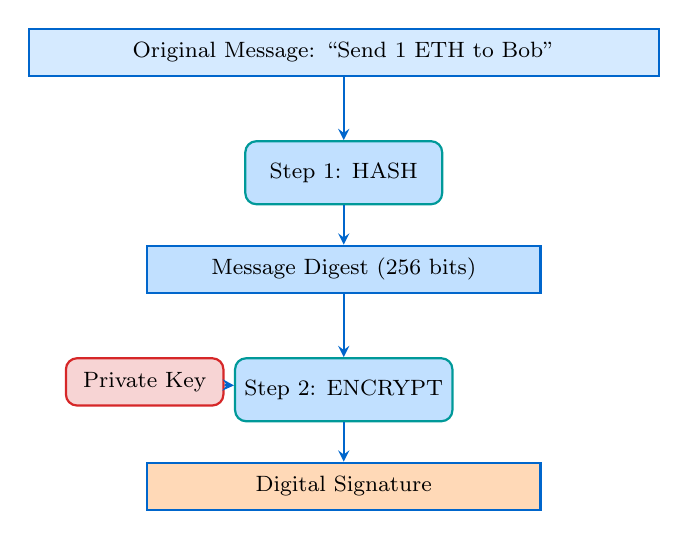
\begin{tikzpicture}[node distance=0.3cm]
% Step 1
\node[databox, minimum width=8cm] (msg) {Original Message: ``Send 1 ETH to Bob''};

% Step 2
\node[hashbox, below=0.8cm of msg, minimum width=2.5cm] (hash) {Step 1: HASH};
\node[databox, below=0.5cm of hash, minimum width=5cm, fill=dflightblue3] (digest) {Message Digest (256 bits)};

% Step 3
\node[keybox, fill=dfred!20, draw=dfred, below left=0.8cm and -1cm of digest] (priv) {Private Key};
\node[hashbox, below=0.8cm of digest, minimum width=2.5cm] (encrypt) {Step 2: ENCRYPT};
\node[databox, below=0.5cm of encrypt, minimum width=5cm, fill=dforange!30] (sig) {Digital Signature};

% Arrows
\draw[arrow] (msg) -- (hash);
\draw[arrow] (hash) -- (digest);
\draw[arrow] (digest) -- (encrypt);
\draw[arrow] (priv) -- (encrypt);
\draw[arrow] (encrypt) -- (sig);
\end{tikzpicture}
\end{center}

\vspace{3mm}
\textbf{Why hash first?}
\begin{itemize}
\item Messages can be any size; hashes are always fixed (256 bits)
\item Encrypting a small hash is much faster than encrypting a large message
\end{itemize}
\end{frame}

% =======================================================================
% SLIDE 22: The Verification Process
% =======================================================================
\begin{frame}{The Verification Process: Step by Step}
\begin{center}
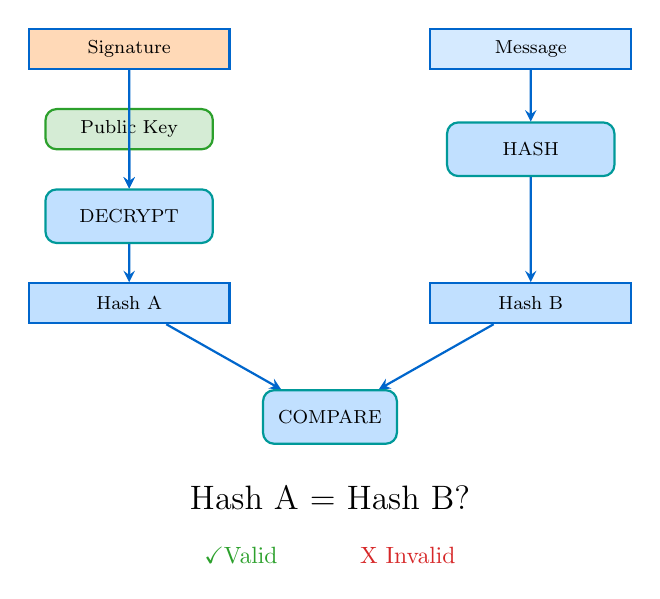
\begin{tikzpicture}[node distance=0.3cm, scale=0.85, transform shape]
% Left path: Decrypt signature
\node[databox, fill=dforange!30, minimum width=3cm] (sig) at (-3,3) {Signature};
\node[keybox, fill=dfgreen!20, draw=dfgreen, minimum width=2.5cm] (pub) at (-3,1.8) {Public Key};
\node[hashbox, minimum width=2.5cm] (decrypt) at (-3,0.5) {DECRYPT};
\node[databox, fill=dflightblue3, minimum width=3cm] (hash1) at (-3,-0.8) {Hash A};

% Right path: Hash message
\node[databox, minimum width=3cm] (msg) at (3,3) {Message};
\node[hashbox, minimum width=2.5cm] (hash) at (3,1.5) {HASH};
\node[databox, fill=dflightblue3, minimum width=3cm] (hash2) at (3,-0.8) {Hash B};

% Compare
\node[hashbox, minimum width=2cm] (compare) at (0,-2.5) {COMPARE};
\node[below=0.5cm of compare] (result) {\Large Hash A = Hash B?};
\node[below=0.3cm of result] {\textcolor{dfgreen}{\checkmark Valid} \hspace{1cm} \textcolor{dfred}{X Invalid}};

% Arrows
\draw[arrow] (sig) -- (decrypt);
\draw[arrow] (pub) -- (decrypt);
\draw[arrow] (decrypt) -- (hash1);
\draw[arrow] (msg) -- (hash);
\draw[arrow] (hash) -- (hash2);
\draw[arrow] (hash1) -- (compare);
\draw[arrow] (hash2) -- (compare);
\end{tikzpicture}
\end{center}

\textbf{If hashes match:} Signature is valid -- message is authentic and unaltered
\end{frame}

% =======================================================================
% SLIDE 23: Digital Signatures in Blockchain
% =======================================================================
\begin{frame}{Digital Signatures in Blockchain Transactions}
Every blockchain transaction includes a digital signature proving authorization:

\vspace{3mm}
\begin{center}
\begin{tabular}{|l|l|}
\hline
\textbf{Field} & \textbf{Value} \\
\hline
From & 0x7a2b...9f3c \\
To & 0x9c4d...e8f2 \\
Value & 1.5 ETH \\
Nonce & 42 \\
Gas Limit & 21,000 \\
Gas Price & 50 gwei \\
\textbf{Signature} & \textit{v, r, s (proves authorization)} \\
\hline
\end{tabular}
\end{center}

\vspace{5mm}
\textbf{How it works in practice:}
\begin{enumerate}
\item Alice creates transaction: ``Send 1.5 ETH to Bob''
\item Alice signs with her private key
\item Network verifies signature using Alice's public key
\item If valid: transaction is processed. If invalid: rejected
\end{enumerate}
\end{frame}

% =======================================================================
% SLIDE 24: Summary - The Cryptographic Trust Stack
% =======================================================================
\begin{frame}{Summary: The Cryptographic Trust Stack}
\begin{center}
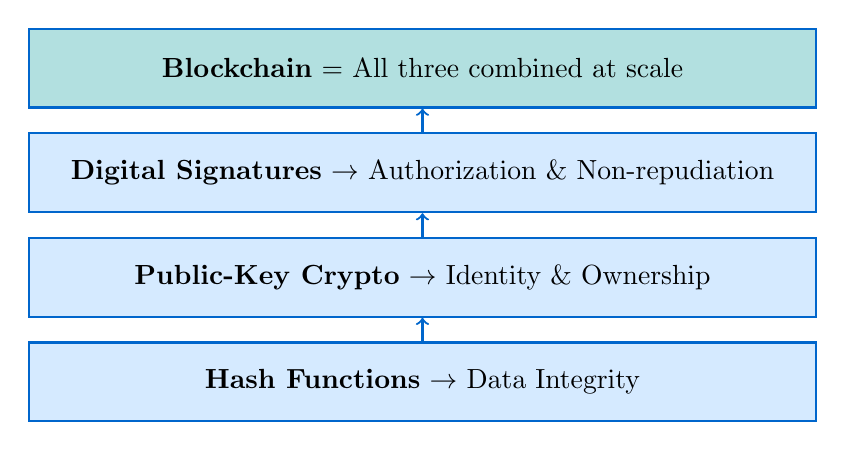
\begin{tikzpicture}[node distance=0.3cm]
% Stack of guarantees
\node[process, minimum width=10cm, minimum height=1cm] (l1) {
\textbf{Hash Functions} $\rightarrow$ Data Integrity
};
\node[process, minimum width=10cm, minimum height=1cm, above=of l1] (l2) {
\textbf{Public-Key Crypto} $\rightarrow$ Identity \& Ownership
};
\node[process, minimum width=10cm, minimum height=1cm, above=of l2] (l3) {
\textbf{Digital Signatures} $\rightarrow$ Authorization \& Non-repudiation
};
\node[process, minimum width=10cm, minimum height=1cm, fill=dfteal!30, above=of l3] (l4) {
\textbf{Blockchain} = All three combined at scale
};

\draw[thick, dfblue, ->] (l1.north) -- (l2.south);
\draw[thick, dfblue, ->] (l2.north) -- (l3.south);
\draw[thick, dfblue, ->] (l3.north) -- (l4.south);
\end{tikzpicture}
\end{center}

\vspace{5mm}
\begin{block}{Key Takeaway}
Cryptography transforms trust from ``believe the institution'' to ``verify the math.''
No bank, government, or third party needed -- just mathematics.
\end{block}
\end{frame}

% =======================================================================
% SLIDE 25: Hands-On Exercise (Part 1)
% =======================================================================
\begin{frame}{Hands-On Exercise: NB05 Cryptographic Operations}
\textbf{What you'll do in the Colab notebook:}

\vspace{3mm}
\begin{enumerate}
\item \textbf{Hash Functions}
\begin{itemize}
\item Compute SHA-256 hashes of different inputs
\item Observe the avalanche effect firsthand
\item Verify that same input = same output
\end{itemize}

\vspace{2mm}
\item \textbf{Key Generation}
\begin{itemize}
\item Generate a public-private key pair
\item Derive a wallet address from the public key
\item Understand the one-way relationship
\end{itemize}

\vspace{2mm}
\item \textbf{Digital Signatures}
\begin{itemize}
\item Sign a message with your private key
\item Verify the signature with the public key
\item See what happens when verification fails
\end{itemize}
\end{enumerate}

\vspace{3mm}
\begin{center}
\fbox{\parbox{0.6\textwidth}{\centering
\textbf{Access:} NB05 -- Cryptographic Operations\\
No installation required (runs in browser)
}}
\end{center}
\end{frame}

% =======================================================================
% SLIDE 26: Hands-On Exercise (Part 2)
% =======================================================================
\begin{frame}[fragile]{Hands-On Preview: Code Snippets}
\textbf{Hashing in Python:}
\begin{lstlisting}[style=pythonstyle, basicstyle=\ttfamily\scriptsize]
import hashlib
message = "Hello, Blockchain!"
hash_result = hashlib.sha256(message.encode()).hexdigest()
print(hash_result)  # 64 hex characters
\end{lstlisting}

\vspace{3mm}
\textbf{Creating a signature:}
\begin{lstlisting}[style=pythonstyle, basicstyle=\ttfamily\scriptsize]
# Sign with private key
signature = private_key.sign(
    message_hash,
    algorithm=hashes.SHA256()
)
\end{lstlisting}

\vspace{3mm}
\textbf{Verifying a signature:}
\begin{lstlisting}[style=pythonstyle, basicstyle=\ttfamily\scriptsize]
# Verify with public key
public_key.verify(signature, message_hash)
# Raises exception if invalid!
\end{lstlisting}

\bottomnote{Complete code and explanations in NB05 notebook}
\end{frame}

% =======================================================================
% SLIDE 27: Discussion - Real-World Applications
% =======================================================================
\begin{frame}{Discussion: Where Do You See These Concepts?}
\textbf{Think-Pair-Share:} Where else are these cryptographic primitives used?

\vspace{5mm}
\begin{columns}[T]
\begin{column}{0.48\textwidth}
\textbf{Hash Functions}
\begin{itemize}
\item Password storage
\item File integrity (checksums)
\item Git version control
\item Digital forensics
\item Deduplication systems
\end{itemize}
\end{column}
\begin{column}{0.48\textwidth}
\textbf{Digital Signatures}
\begin{itemize}
\item Software updates
\item Email (S/MIME, PGP)
\item PDF documents
\item Code signing
\item SSL/TLS certificates
\end{itemize}
\end{column}
\end{columns}

\vspace{5mm}
\begin{block}{Discussion Questions}
\begin{enumerate}
\item Why might a company hash passwords instead of encrypting them?
\item What happens to digital signatures if quantum computers become powerful?
\end{enumerate}
\end{block}
\end{frame}

% =======================================================================
% SLIDE 28: Application - Transaction Security
% =======================================================================
\begin{frame}{Application: How a Blockchain Transaction Stays Secure}
\begin{center}
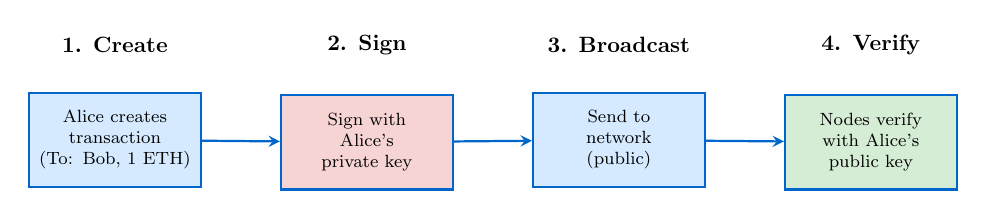
\begin{tikzpicture}[node distance=0.5cm, scale=0.8, transform shape]
% Timeline
\node[font=\bfseries] (t1) at (0,0) {1. Create};
\node[font=\bfseries] (t2) at (4,0) {2. Sign};
\node[font=\bfseries] (t3) at (8,0) {3. Broadcast};
\node[font=\bfseries] (t4) at (12,0) {4. Verify};

% Boxes below
\node[databox, below=0.5cm of t1, text width=2.5cm, align=center, minimum height=1.5cm] (b1) {
Alice creates\\transaction\\(To: Bob, 1 ETH)
};
\node[databox, below=0.5cm of t2, text width=2.5cm, align=center, minimum height=1.5cm, fill=dfred!20] (b2) {
Sign with\\Alice's\\private key
};
\node[databox, below=0.5cm of t3, text width=2.5cm, align=center, minimum height=1.5cm] (b3) {
Send to\\network\\(public)
};
\node[databox, below=0.5cm of t4, text width=2.5cm, align=center, minimum height=1.5cm, fill=dfgreen!20] (b4) {
Nodes verify\\with Alice's\\public key
};

% Arrows
\draw[arrow] (b1) -- (b2);
\draw[arrow] (b2) -- (b3);
\draw[arrow] (b3) -- (b4);
\end{tikzpicture}
\end{center}

\vspace{3mm}
\textbf{Security guarantees at each step:}
\begin{itemize}
\item \textbf{Step 2:} Only Alice can sign (private key)
\item \textbf{Step 3:} Transaction is public but tamper-evident (hash)
\item \textbf{Step 4:} Anyone can verify Alice authorized it (public key)
\end{itemize}

\textcolor{dfblue}{\textbf{Result:}} No one can forge, alter, or deny the transaction
\end{frame}

% =======================================================================
% SLIDE 29: Application - Multi-Signature Wallets
% =======================================================================
\begin{frame}{Application: Multi-Signature Wallets}
\textbf{Problem:} What if one private key is stolen or lost?

\vspace{3mm}
\textbf{Solution:} Require multiple signatures (e.g., 2-of-3 multisig)

\begin{center}
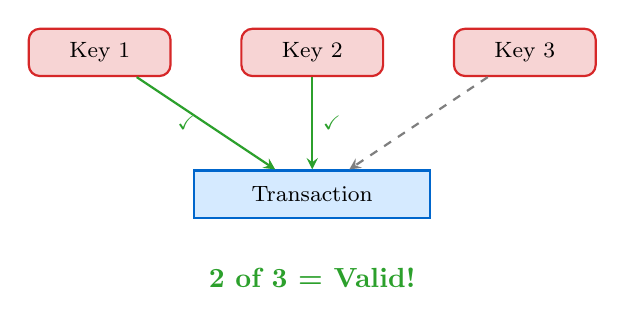
\begin{tikzpicture}[scale=0.9]
% Three keys
\node[keybox, fill=dfred!20, draw=dfred, minimum width=1.8cm] (k1) at (0,2) {Key 1};
\node[keybox, fill=dfred!20, draw=dfred, minimum width=1.8cm] (k2) at (3,2) {Key 2};
\node[keybox, fill=dfred!20, draw=dfred, minimum width=1.8cm] (k3) at (6,2) {Key 3};

% Transaction
\node[databox, minimum width=3cm] (tx) at (3,0) {Transaction};

% Arrows
\draw[arrow, dfgreen] (k1) -- node[left, font=\scriptsize] {\checkmark} (tx);
\draw[arrow, dfgreen] (k2) -- node[right, font=\scriptsize] {\checkmark} (tx);
\draw[arrow, dashed, dfgray] (k3) -- (tx);

% Result
\node[below=0.5cm of tx, text=dfgreen, font=\bfseries] {2 of 3 = Valid!};
\end{tikzpicture}
\end{center}

\vspace{3mm}
\textbf{Use Cases:}
\begin{itemize}
\item Corporate treasury (CFO + CEO approval)
\item Family inheritance (multiple heirs)
\item Exchange cold storage (security team)
\end{itemize}

\bottomnote{Multi-sig combines multiple digital signatures for enhanced security}
\end{frame}

% =======================================================================
% SLIDE 30: Application - Trust Implications
% =======================================================================
\begin{frame}{Application: Trust Implications for Finance}
\textbf{How cryptography changes financial trust:}

\vspace{3mm}
\begin{center}
\begin{tabular}{lcc}
\toprule
\textbf{Aspect} & \textbf{Traditional} & \textbf{Cryptographic} \\
\midrule
Identity verification & Bank/Government & Public key \\
Authorization & Signature card & Digital signature \\
Transaction integrity & Bank records & Hash chains \\
Dispute resolution & Courts & Mathematical proof \\
Account recovery & ID documents & Seed phrase \\
\bottomrule
\end{tabular}
\end{center}

\vspace{5mm}
\begin{block}{Trade-off}
\textbf{Benefit:} No intermediaries, censorship-resistant, 24/7 operation\\
\textbf{Risk:} ``With great power comes great responsibility'' -- lose your keys, lose your funds
\end{block}
\end{frame}

% =======================================================================
% SLIDE 31: Executive Summary
% =======================================================================
\begin{frame}{Executive Summary: 5 Key Takeaways}
\begin{enumerate}
\item \textbf{Hash functions} create unique digital fingerprints -- any change to data produces a completely different hash, enabling tamper detection

\vspace{3mm}
\item \textbf{Public-key cryptography} allows secure identity without central authorities -- you control your identity through your private key

\vspace{3mm}
\item \textbf{Digital signatures} provide three guarantees: authentication (who signed), integrity (not altered), and non-repudiation (can't deny signing)

\vspace{3mm}
\item \textbf{These primitives combine} in blockchain to enable trustless transactions -- math replaces institutional trust

\vspace{3mm}
\item \textbf{Security responsibility shifts} from institutions to individuals -- ``not your keys, not your coins''
\end{enumerate}
\end{frame}

% =======================================================================
% SLIDE 32: Concept Map
% =======================================================================
\begin{frame}{Concept Map: How It All Connects}
\begin{center}
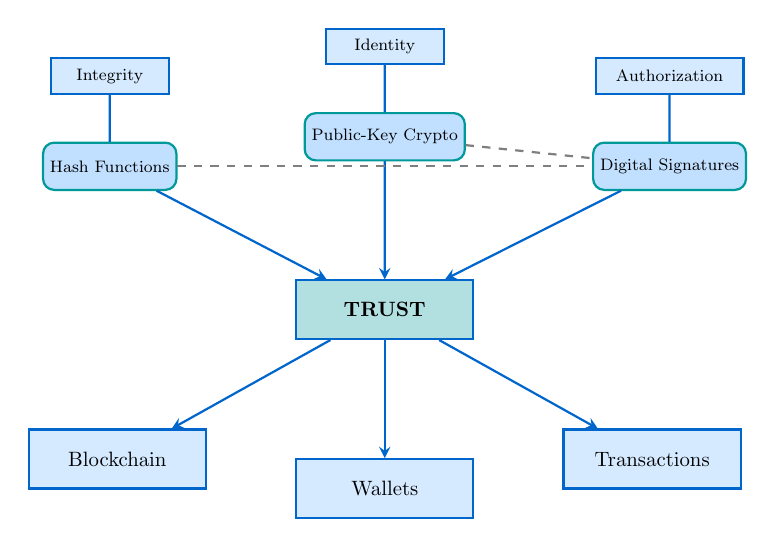
\begin{tikzpicture}[node distance=1.5cm, scale=0.75, transform shape]
% Central node
\node[process, fill=dfteal!30, minimum width=3cm] (trust) at (0,0) {\textbf{TRUST}};

% Three primitives
\node[hashbox, above left=1.5cm and 2cm of trust] (hash) {Hash Functions};
\node[hashbox, above=2cm of trust] (pubkey) {Public-Key Crypto};
\node[hashbox, above right=1.5cm and 2cm of trust] (sig) {Digital Signatures};

% What they provide
\node[databox, above=0.8cm of hash, minimum width=2cm] (integ) {Integrity};
\node[databox, above=0.8cm of pubkey, minimum width=2cm] (ident) {Identity};
\node[databox, above=0.8cm of sig, minimum width=2.5cm] (auth) {Authorization};

% Lower applications
\node[process, below left=1.5cm and 1.5cm of trust] (block) {Blockchain};
\node[process, below=2cm of trust] (wallet) {Wallets};
\node[process, below right=1.5cm and 1.5cm of trust] (tx) {Transactions};

% Connections to trust
\draw[arrow] (hash) -- (trust);
\draw[arrow] (pubkey) -- (trust);
\draw[arrow] (sig) -- (trust);

% Connections from trust
\draw[arrow] (trust) -- (block);
\draw[arrow] (trust) -- (wallet);
\draw[arrow] (trust) -- (tx);

% Connections to properties
\draw[thick, dfblue] (hash) -- (integ);
\draw[thick, dfblue] (pubkey) -- (ident);
\draw[thick, dfblue] (sig) -- (auth);

% Cross connections
\draw[thick, dfgray, dashed] (hash) -- (sig);
\draw[thick, dfgray, dashed] (pubkey) -- (sig);
\end{tikzpicture}
\end{center}

\vspace{2mm}
\textbf{Key relationship:} Digital signatures combine hash functions (for efficiency) with public-key crypto (for authentication)
\end{frame}

% =======================================================================
% SLIDE 33: Key Terms & Definitions (Part 1)
% =======================================================================
\begin{frame}{Key Terms \& Definitions (Part 1)}
\begin{description}
\item[Hash Function] A mathematical function that converts any input into a fixed-size output (digest). One-way and deterministic.

\vspace{2mm}
\item[SHA-256] Secure Hash Algorithm producing 256-bit output. Used in Bitcoin and many blockchains.

\vspace{2mm}
\item[Avalanche Effect] Property where a tiny input change causes a dramatically different output hash.

\vspace{2mm}
\item[Collision Resistance] Property that makes it computationally infeasible to find two different inputs with the same hash.

\vspace{2mm}
\item[Merkle Tree] A tree structure where each leaf is a hash of data, and each non-leaf is a hash of its children. Enables efficient verification.
\end{description}
\end{frame}

% =======================================================================
% SLIDE 34: Key Terms & Definitions (Part 2)
% =======================================================================
\begin{frame}{Key Terms \& Definitions (Part 2)}
\begin{description}
\item[Public Key] The shareable part of a key pair, used to verify signatures or encrypt messages.

\vspace{2mm}
\item[Private Key] The secret part of a key pair, used to create signatures or decrypt messages. Must never be shared.

\vspace{2mm}
\item[Digital Signature] Cryptographic proof that a message was approved by the holder of a specific private key.

\vspace{2mm}
\item[ECDSA] Elliptic Curve Digital Signature Algorithm. Used by Bitcoin and Ethereum for smaller, faster signatures.

\vspace{2mm}
\item[Non-repudiation] The property that a signer cannot deny having signed a message, as only their private key could have created the signature.
\end{description}
\end{frame}

% =======================================================================
% SLIDE 35: Common Misconceptions
% =======================================================================
\begin{frame}{Common Misconceptions: Myth vs Reality}
\begin{columns}[T]
\begin{column}{0.48\textwidth}
\textbf{\textcolor{dfred}{Myth 1:}}\\
``Hashing encrypts data''

\textbf{\textcolor{dfgreen}{Reality:}}\\
Hashing is one-way -- you cannot ``decrypt'' a hash. Encryption is reversible; hashing is not.

\vspace{5mm}
\textbf{\textcolor{dfred}{Myth 2:}}\\
``If my public key is exposed, I'm hacked''

\textbf{\textcolor{dfgreen}{Reality:}}\\
Public keys are \textit{meant} to be public! Only exposure of your private key is dangerous.
\end{column}
\begin{column}{0.48\textwidth}
\textbf{\textcolor{dfred}{Myth 3:}}\\
``Longer passwords = stronger hashes''

\textbf{\textcolor{dfgreen}{Reality:}}\\
Hash output size is fixed regardless of input. A 256-bit hash is 256 bits whether input is ``a'' or a novel.

\vspace{5mm}
\textbf{\textcolor{dfred}{Myth 4:}}\\
``Quantum computers will break all crypto''

\textbf{\textcolor{dfgreen}{Reality:}}\\
Some algorithms are vulnerable, but post-quantum cryptography already exists. Hash functions remain largely secure.
\end{column}
\end{columns}
\end{frame}

% =======================================================================
% SLIDE 36: Self-Assessment Questions (Part 1)
% =======================================================================
\begin{frame}{Self-Assessment: Test Your Understanding}
\textbf{Question 1:} What is the primary purpose of a cryptographic hash function?

\vspace{2mm}
\begin{enumerate}[A.]
\item To encrypt data so it can be decrypted later
\item To create a fixed-size unique fingerprint of any input data
\item To generate random numbers for cryptographic operations
\item To compress large files into smaller ones
\end{enumerate}

\vspace{5mm}
\pause
\textbf{Answer: B}

A cryptographic hash function takes any input and produces a fixed-size output called a hash or digest. This serves as a unique ``fingerprint'' of the data. Unlike encryption, hashing is one-way and cannot be reversed.
\end{frame}

% =======================================================================
% SLIDE 37: Self-Assessment Questions (Part 2)
% =======================================================================
\begin{frame}{Self-Assessment: Test Your Understanding}
\textbf{Question 2:} What three properties does a digital signature provide?

\vspace{2mm}
\begin{enumerate}[A.]
\item Encryption, compression, and speed
\item Authentication, integrity, and non-repudiation
\item Confidentiality, availability, and scalability
\item Hashing, signing, and verification
\end{enumerate}

\vspace{3mm}
\pause
\textbf{Answer: B}

A digital signature provides: (1) \textbf{Authentication} -- proves who signed, (2) \textbf{Integrity} -- proves the message wasn't altered, and (3) \textbf{Non-repudiation} -- the signer cannot deny having signed.

\vspace{3mm}
\hrule
\vspace{3mm}
\textbf{Question 3:} What is the ``birthday attack'' in hash functions?

\pause
Finding a collision requires only $2^{128}$ attempts for SHA-256 (not $2^{256}$) due to probability theory -- still astronomically large but worth knowing!
\end{frame}

% =======================================================================
% SLIDE 38: What's Next
% =======================================================================
\begin{frame}{What's Next: Topic 3.2 -- Blockchain Mechanics}
\textbf{Now that you understand the building blocks, we'll see how they assemble:}

\vspace{5mm}
\begin{columns}[T]
\begin{column}{0.48\textwidth}
\textbf{Topics Covered:}
\begin{itemize}
\item What is a blockchain?
\item How blocks link together
\item The block structure
\item Consensus mechanisms
\item The blockchain trilemma
\end{itemize}
\end{column}
\begin{column}{0.48\textwidth}
\textbf{You'll Learn:}
\begin{itemize}
\item Why tampering is detectable
\item How networks agree on truth
\item Trade-offs in blockchain design
\item Proof of Work vs Proof of Stake
\end{itemize}
\end{column}
\end{columns}

\vspace{5mm}
\begin{center}
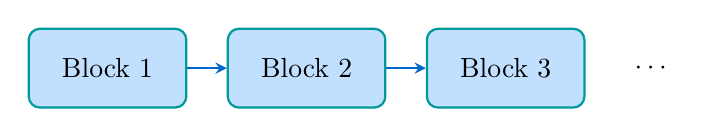
\begin{tikzpicture}
\node[blockchain, minimum width=2cm] (b1) {Block 1};
\node[blockchain, minimum width=2cm, right=0.5cm of b1] (b2) {Block 2};
\node[blockchain, minimum width=2cm, right=0.5cm of b2] (b3) {Block 3};
\node[right=0.5cm of b3] {$\cdots$};
\draw[arrow] (b1) -- (b2);
\draw[arrow] (b2) -- (b3);
\end{tikzpicture}
\end{center}

\bottomnote{Preview: The hash of each block is included in the next -- creating an unbreakable chain}
\end{frame}

% =======================================================================
% SLIDE 39: Resources
% =======================================================================
\begin{frame}{Resources for Further Learning}
\textbf{Hands-On:}
\begin{itemize}
\item \textbf{NB05:} Cryptographic Operations (Colab notebook)
\item Online SHA-256 calculator: \url{https://emn178.github.io/online-tools/sha256.html}
\end{itemize}

\vspace{3mm}
\textbf{Reading:}
\begin{itemize}
\item Antonopoulos, A. (2017). \textit{Mastering Bitcoin}, Chapter 4: Keys \& Addresses
\item Narayanan et al. (2016). \textit{Bitcoin and Cryptocurrency Technologies}, Chapter 1
\end{itemize}

\vspace{3mm}
\textbf{Video:}
\begin{itemize}
\item 3Blue1Brown: ``How secure is 256-bit security?'' (YouTube)
\item Computerphile: ``Hashing Algorithms and Security'' (YouTube)
\end{itemize}

\vspace{3mm}
\textbf{Interactive:}
\begin{itemize}
\item Anders Brownworth's Blockchain Demo: \url{https://andersbrownworth.com/blockchain/}
\end{itemize}
\end{frame}

% =======================================================================
% SLIDE 40: Questions Closing Slide
% =======================================================================
\begin{frame}
\begin{center}
\vspace{1cm}
{\Huge \textcolor{dfblue}{Questions?}}

\vspace{1.5cm}
{\Large Topic 3.1: Cryptographic Building Blocks}

\vspace{1cm}
{\large Hashing, Keys, and Digital Signatures}

\vspace{1.5cm}
\textbf{Next:} Topic 3.2 -- Blockchain Mechanics

\vspace{1cm}
\textcolor{dfgray}{\small Joerg Osterrieder | Digital Finance | 2025}
\end{center}
\end{frame}

\end{document}
